\section{Registration of Acquisitions}
\label{section:acquisition-registration}

During a capture, multiple acquisitions are performed and to each one corresponds a transformation (position and orientation) to the scene referencial. In this section, a method is described to find each one of this transformations, so all the acquisitions are merged into a single point cloud. The method chosen is the Iterative Closest Point, or ICP. This method is capable of aligning two point clouds, the reference and the target point cloud, by finding the transformation between the second to the first one. This is also known as point cloud registration.

\subsection{Iterative Closest Point}

\newcommand{\T}{\mathrm{T}}
\newcommand{\Pt}{\mathcal{P}}
\newcommand{\Q}{\mathcal{Q}}

Iterative Closest Point, or ICP, is a method which finds the transformation between two pont clouds: a reference point cloud and a target point cloud, by minimizing the distance between correspondent features, as points, lines or edges, found in both point clouds. A further explanation of the process can be found in \cite{besl92}.

This method can be divided in two steps: the correspondence or matching steps, which finds the common features between the point clouds and the iterative optimization step, which find the transformation though an optimization algorithm. Multiple improvements can be made to the algorithm, by choosing different optimizations or correspondent algorithms. A common modification, for example, is to remove the outliers features which have no correspondence.

A common problem of this method is an imperfect correspondence, which compromises the final result. This is greater if the point clouds are not dense and if there is small overlap between them. In general, point-to-point correspondent is not very robust. To overcome this problem, it is common to use more robust features, like visual features, for example markers, or geometric features, for example corners.

In this work, a simple ICP method with a point-to-point correspondence algorithm with outlier removal was used.

\subsection{ICP for Multiple Point Clouds}
\label{section:multiple-pointcloud-icp}

ICP can only register pairs of point clouds, whereas this work requires a registration of $N$ point clouds, corresponding to $n$ acquisitions. So, a technique has to be found so that the ICP algorithm can be used with $n$ point clouds. Three of this techniques are now described, ordered by their complexity:

\begin{itemize}
    \item The first approach and the easier one to implement is to register each point clouds sequencially. In other words, this method registers the point cloud $\Pt_i$ to the point cloud $\Pt_{i-1}$ and the transformation $\T_{i-1}^{i}$ is found. The final accumulated point cloud is assembled using the \cref{eqn:registration-simple-method-calculation}. This method is the one that requires less overall registration, but has the disadvantage that the accumulative transformation errors increases for each successive point cloud. This approach is shown in \cref{figure:registration-methods-approaches}.
    \begin{equation}
        \label{eqn:registration-simple-method-calculation}
            \Pt = \bigcup{\left(\T_1^2 \circ \T_2^3 \circ \dots \circ \T_{i-1}^i\right)(\Pt_i)}
    \end{equation}

    \item The next approach is widely used in robotics for Simultaneous Location and Mapping , or SLAM. This method holds an accumulated point cloud $A$ in memory, and each new incoming point cloud $\Pt$ registers to the accumulated point cloud.  Afterwards it is merged into $A$, which is then used for the next iteration, as shown in \cref{figure:registration-methods-approaches}. It has the advantage that each new registration is done against a wider point cloud so there is more overlapping between the point clouds. Also, at each iteration the current pose of the 3D scanner is obtained, which is used as an initial estimate for the next iteration. However, the accumulated point cloud grows at each iteration, and some filtering has to be performed to maintain the number of points bounded. In conclusion, each iteration can be calculated as:
    
    \begin{align}
        \label{eqn:icp-compose-1}
        \T_{i} = & \textrm{ICP}(A, \Pt_{i}, \T_0 = \T_{i-1}), \\
        \label{eqn:icp-compose-2}
        A_{i+1} = & A{i} \bigcup \T_{i}(\Pt_i).
    \end{align}

    \item The last approach is the most complex. The idea of this approach is to minimize the number of transformation combinations, to minimize the propagation of the error. In particular, the registrations for the $N$ points clouds are done pairwise and are merged together to create a new point cloud. Then, this process is done recursively until an unique point cloud is obtained. This way, the maximum number of transformation combinations are equal to the number of levels of the tree, which is $\log_2(N)$, instead of $N$ combinations in the first approach. This algorithm is formalized in \cref{eqn:registration-tree-method-1,eqn:registration-tree-method-2}, for a list of point clouds $S=\left\{P_1, P_2, \ \dots, \ P_n\right\}$. At each level $l$ a new list of point clouds $^{l}P$ and transformations $^{l}T$ are computed, as shown in \cref{figure:registration-methods-approaches}:

    \begin{align}
        ^{l}\T = & \left\{\textrm{ICP}(^{l-1}\Pt_1, ^{l-1}\Pt_2), \ \dots, \ \textrm{ICP}(^{l-1}\Pt_{n-1}, ^{l-1}\Pt_{n}) \right\},
            \label{eqn:registration-tree-method-1} \\
        ^{l}\Pt = & \left\{^{l-1}\Pt_1 \bigcup{^{l}\T_1(^{l-1}\Pt_2}), \ \dots, \ ^{l-1}\Pt_{n-1} \bigcup{^{l}\T_{n/2}(^{l-1}\Pt_n)}\right\}.
            \label{eqn:registration-tree-method-2}
    \end{align}
    
\end{itemize}

In conclusion, three methods are possible to extend the ICP algorithm to multiple point clouds, and the three methods were used in this work and compared. After this registration the point clouds are assembled into the final point cloud. There is, however, a limitation of all this methods, because all of them have the principle that every point cloud is close to the previous one, which can be false. In this work, this was ensured in the capture methodology. 

\begin{figure}
    \centering
    \begin{subfigure}[t]{0.3\textwidth}
        \centering
        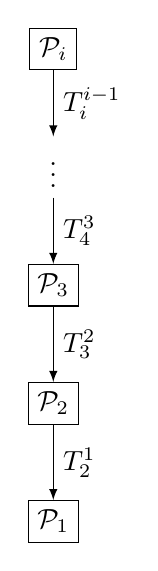
\begin{tikzpicture}
            \node[draw] (P1) at (0,0) {$\Pt_1$};
            \node[draw] (P2) at (0,1.5) {$\Pt_2$};
            \node[draw] (P3) at (0,3) {$\Pt_3$};
            \node (P4) at (0,4.5) {$\vdots$};
            \node[draw] (Pi) at (0,6) {$\Pt_i$};

            \draw[-latex] (P2) -- (P1) node[midway, anchor=west] {$T_2^1$};
            \draw[-latex] (P3) -- (P2) node[midway, anchor=west] {$T_3^2$};
            \draw[-latex] (P4) -- (P3) node[midway, anchor=west] {$T_4^3$};
            \draw[-latex] (Pi) -- (P4) node[midway, anchor=west] {$T_i^{i-1}$};
        \end{tikzpicture}

        \caption{First method.}
        \label{figure:multiple-icp-method-1}
    \end{subfigure}%
    \begin{subfigure}[t]{0.3\textwidth}
        
        \centering
        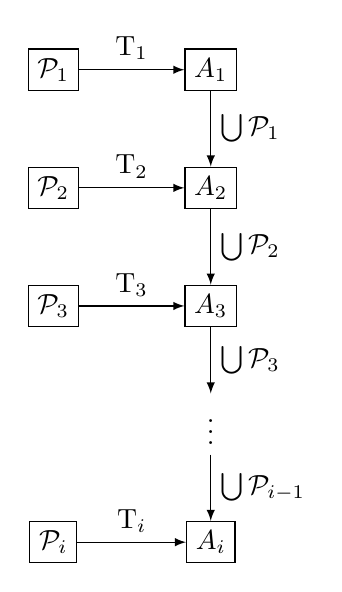
\begin{tikzpicture}
            \node[draw] (A1) at (0,0) {$A_1$};
            \node[draw] (A2) at (0,-1.5) {$A_2$};
            \node[draw] (A3) at (0,-3) {$A_3$};
            \node (A4) at (0,-4.5) {$\vdots$};
            \node[draw] (Ai) at (0,-6) {$A_i$};

            \node[draw, left of=A1, xshift=-1cm] (P1) {$\Pt_1$};
            \draw[-latex] (P1) -- (A1) node[midway, above] {$\T_1$};

            \node[draw, left of=A2, xshift=-1cm] (P2) {$\Pt_2$};
            \draw[-latex] (P2) -- (A2) node[midway, above] {$\T_2$};

            \node[draw, left of=A3, xshift=-1cm] (P3) {$\Pt_3$};
            \draw[-latex] (P3) -- (A3) node[midway, above] {$\T_3$};

            \node[draw, left of=Ai, xshift=-1cm] (Pi) {$\Pt_i$};
            \draw[-latex] (Pi) -- (Ai) node[midway, above] {$\T_i$};

            \draw[-latex] (A1) -- (A2) node[midway, right] {$\bigcup{\Pt_1}$};
            \draw[-latex] (A2) -- (A3) node[midway, right] {$\bigcup{\Pt_2}$};
            \draw[-latex] (A3) -- (A4) node[midway, right] {$\bigcup{\Pt_3}$};
            \draw[-latex] (A4) -- (Ai) node[midway, right] {$\bigcup{\Pt_{i-1}}$};
        \end{tikzpicture}

        \caption{Second method.}
        \label{figure:multiple-icp-method-2}
    \end{subfigure}%
    \begin{subfigure}[t]{0.4\textwidth}
        
        \centering
        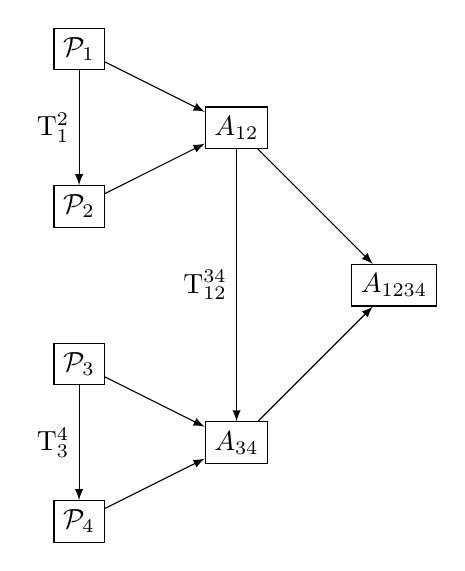
\begin{tikzpicture}
            \node[draw] (P1) at (0,0)  {$\Pt_1$};
            \node[draw] (P2) at (0,-2) {$\Pt_2$};
            \node[draw] (P3) at (0,-4) {$\Pt_3$};
            \node[draw] (P4) at (0,-6) {$\Pt_4$};

            \node[draw] (A12) at (2, -1) {$A_{12}$};
            \node[draw] (A34) at (2, -5) {$A_{34}$};
            \node[draw] (A1234) at (4, -3) {$A_{1234}$};

            \draw[-latex] (P1) -- (A12);
            \draw[-latex] (P2) -- (A12);
            \draw[-latex] (P3) -- (A34);
            \draw[-latex] (P4) -- (A34);
            \draw[-latex] (A12) -- (A1234);
            \draw[-latex] (A34) -- (A1234);

            \draw[-latex] (P1) -- (P2) node[midway, left] {$\T_1^2$};
            \draw[-latex] (P3) -- (P4) node[midway, left] {$\T_3^4$};
            \draw[-latex] (A12) -- (A34) node[midway, left] {$\T_{12}^{34}$};

        \end{tikzpicture}
        \caption{Third method.}
        \label{figure:multiple-icp-method-3}
    \end{subfigure}%


    \caption{Multiple Point Cloud ICP approaches.}
    \label{figure:registration-methods-approaches}
\end{figure}